\chapter{How to use this book}

The idea of this method is to give you the tools to be creative with music. Concretely this means that instead of saying "The D chord is played using this shape", the following will be said: "A chord is constructed like \textit{this}. So to play a D chord do \textit{this} and you will end up with this shape". Where the "\textit{this}" is some knowledge you will learn.

During the method you will notice that you will see certain constructs/symbols/etc. that you may not know yet and that are not explained directly. This is with intention. The idea is that by exposing you early on to something, while not consciously needing it yet, it is easier to learn the meaning of it later on.

When putting it in steps it looks as follows:

\begin{enumerate}
	\item Expose you to new concepts so you have seen it, but not necessarily understand it yet.
	\item Guided by exercises and songs, explain the previously shown concepts and how they work together.
	\item Understand the theory of the concepts and be able to use them in playing.
	\item Start at 1. again with new concepts.
\end{enumerate}

\autoref{fig:guitar_book_build_up} illustrates the main building blocks of this method. The book starts at the bottom row (the fundamentals) and builds up from there.

\begin{figure}[!b]
	\centering
	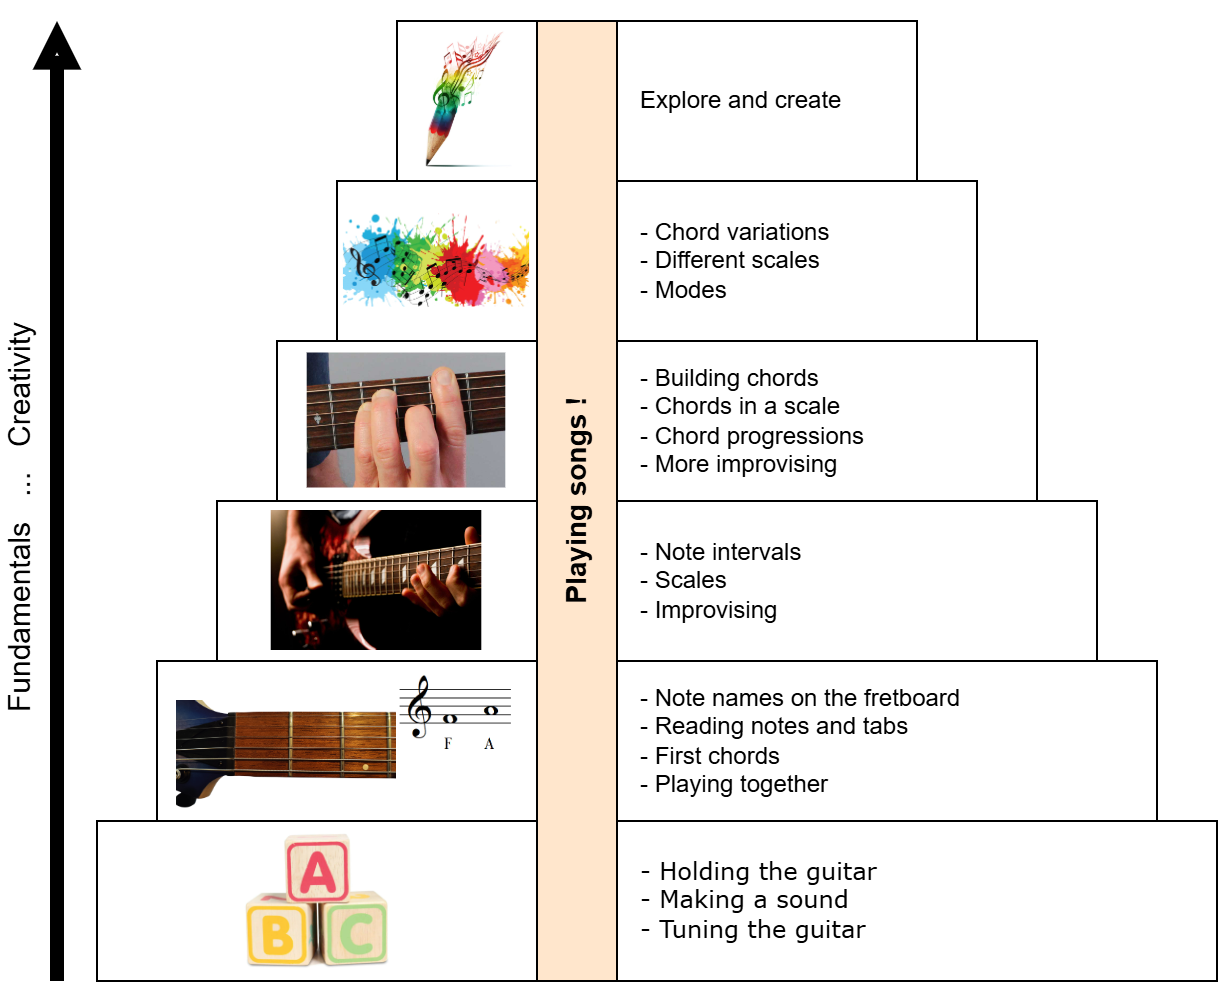
\includegraphics[width=0.85\textwidth]{../../Images/BookBuildup.png}
	\caption{General building blocks of this book}
	\label{fig:guitar_book_build_up}
\end{figure}

\newpage

The fretboard diagrams are drawn such that the \textbf{thickest string is at the bottom}. This resembles the way that you look at the neck when you are holding the guitar.

The chord charts will be shown either with or without the open strings being shown (\autoref{fig:open_chord_chart_example} and \autoref{fig:closed_chord_chart_example} respectively). The fret numbers shown at the bottom are in the same position that you would find fret indications on the guitar neck.

The \textbf{green notes} indicate the root note. The \textbf{orange notes} are the rest of the notes in the chord. The \textbf{gray "X"} means to not play, or to mute, this note/string.

\begin{figure}[h]
	\begin{subfigure}[b]{0.45\textwidth}
		\centering
		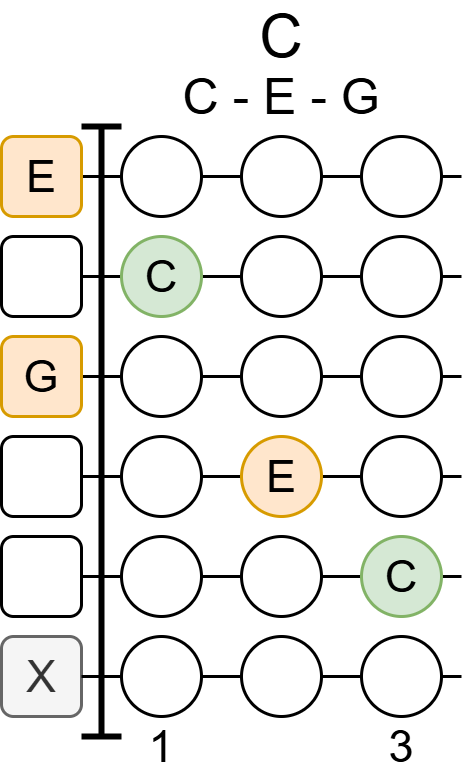
\includegraphics[height=0.3\textheight]{../../Images/OpenCChordChart.png}
		\caption{Open-C chord chart}
		\label{fig:open_chord_chart_example}
	\end{subfigure}
	\hfill
	\begin{subfigure}[b]{0.45\textwidth}
		\centering
		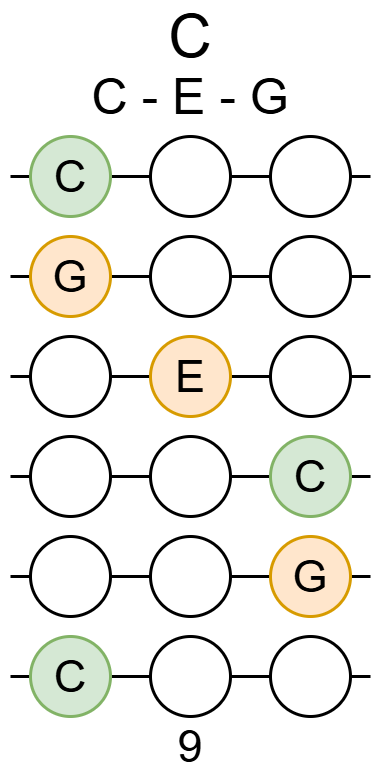
\includegraphics[height=0.3\textheight]{../../Images/ClosedCChordChart.png}
		\caption{Closed-C chord chart}
		\label{fig:closed_chord_chart_example}
	\end{subfigure}
	\caption{Different kinds of chord charts used in this book}
	\label{fig:kinds_of_chord_charts_in_the_book}
\end{figure}